\chapter{Intrinsic stellar variability}
\label{chapISV}
Once a potential host star has been identified, additional criteria determine if it is possible to detect the presence of an exoplanet. Variability is of particular significance when detecting low-mass planets, especially around small, dim stars like M-dwarfs, as the exoplanets influence on the Doppler velocity of the star could be so weak as to be buried in the noise of the variability. If a star is too variable, the presence of an exoplanet would be undetectable, and it would be pointless to include it in a low-mass exoplanet survey. As mentioned in Section\,\ref{SecVarMeth}, the standard method for measuring is an activity index - looking at the variation over time of flux present in lines known to be strongly influenced by variability. This is useful for stars that emit sufficient flux in those lines. However, for cooler stars, like M-dwarfs, that emit mostly in the red, the commonly used lines are less useful and replacements are required.\\

A method that leverages the lines most commonly found in cool stars could provide a better measure on activity as they will be more sensitive to changes in the photosphere. Specifically the molecular TiO and VO lines that are abundant across large sections of the wavelength range. Since an activity index is essentially the ratio of an active line's strength and the nearby continuum, it would be difficult to apply to a single molecular line for two reasons:\\

First, it will be complicated to accurately measure the flux to determine the index. As changes in a line's profile can appear at any part of the line profile, we usually measure the flux across a generous wavelength range, to ensure we account for the whole line. Molecular lines are densely packed into bands, making them difficult to resolve individually. Due to this, the contribution of flux from a line profile's wings would be obscured by the adjacent lines. Additionally the continuum levels have to be taken from a region clear of lines. As the molecular lines are tightly packed, the closest clear region might be tens of angstroms away, in a region where the, due to the shape of the black-body profile, the continuum could be significantly different from near the line of interest.\\

The second issue is that the molecular lines have weak intensities, especially compared to the traditional activity indicators. This mean the signal-to-noise of the index would be quite low. Any changes in the line profile would be small as a result, and difficult to measure.\\

Instead of measuring variability from the change in flux over time in one, or a few, lines, a potentially better method would be to measure activity across the entire continuum. As well as avoiding the issues mentioned above, the activity would be measured in the orders used to obtain Doppler velocity. Some orders have small regions of telluric lines, which can be removed from any Doppler velocity analysis. Other orders are dominated by tellurics, making them useless for Doppler analysis, and are avoided. For example, the HARPS orders that contain the H\,$\alpha$ and Na$_{I}$\,D lines are surrounded by regions of telluric lines. While these orders are used for activity analysis, they are not used for exoplanet Doppler velocity studies. A method of measuring activity in the same orders that are used to measure Doppler velocity would be expected to provide activity information in the wavelength regions of most importance for exoplanet Doppler velocity detection.\\

This new method focuses on the the amount that each pixel in an order deviates from the mean, over time. Pixels with a significant deviation are then cross-correlated with the each observation's spectra to obtain the total deviation across an order. Summing all orders gives the total deviation for a particular observation.

\section{The HARPS M-dwarf catalogue}
\label{secHARPS}
For this work, I needed a set of M-dwarf spectra that was of high quality, i.e. high signal-to-noise and resolution, well sampled, and was produced by the same telescope and spectrograph, to keep conditions consistent. The ESO HARPS data fits each of these criteria and is publicly available after a 1-year embargo. All available observations of M-dwarfs observed by HARPS were downloaded. See \,\citep{2013Bonfils} for details in the HARPS M-dwarf sample. Each observation required information from the extracted one dimensional (\_s1d\_) and two-dimensional (\_e2ds\_) spectra and the cross-correlation function (\_ccf\_). Because of this, only observations with all three files were included. The sample is presented in Table\,\ref{tabHARPS}. Spectral classes were taken from the SIMBAD astronomical database \footnote{http://simbad.u-strasbg.fr/simbad/}, and the exoplanet count was taken from the NASA Exoplanet archive \footnote{https://exoplanetarchive.ipac.caltech.edu/}. The number of observations is all observations that meet the criterion of having all three file types as mentioned above, and the criteria discussed in Section\,\ref{secCriteria}.\\

\section{Determining the variability}
\label{secISV}
For each observation ($I$; Figure\,\ref{figLPV_I}), the spectra needs to be reduced, intensities converted from ADU to electrons, and cosmic rays removed. For most stars, the spectra would not need correcting for Doppler velocity shifts as any shift due to the presence of an exoplanet will be small (\textless\,100 ms$^{-1}$), which corresponds to a fraction of one HARPS pixel (700-950 ms$^{-1}$). However for binary stars, the motion of the target around it's centre of mass can be significant and therefore had to be accounted for. Because of this, the spectra was corrected for both barycentric motion and Doppler velocity. In the case of the HARPS M-dwarfs, the required information was provided in the FITS header of the observations and CCFs and the barycentric correction was determined using \textit{barycorr} \citep{2014Wright}.\\

\begin{figure}
	\centering
	\captionsetup{width=.8\textwidth}
    \includegraphics[width=0.8\textwidth]{LPV_I.png}
    \caption{Example HARPS spectra ($I$) of the 46th order of GL551.}
    \label{figLPV_I}
\end{figure}

To properly identify variations in the spectra over time, the spectra requires the same profile across all observations. In most cases the spectra is divided by the blaze function of the spectrograph. However, the black body profile of the star will vary, depending on its spectral class, and each observation can have a slightly different profile, due to the observations being taken at different times, and therefore barycentric effects will vary. To properly prepare the spectra for comparison, the observation-to-observation differences need to be removed.\\

\begin{figure}
    \centering
    \captionsetup{width=.8\textwidth}
    \includegraphics[width=0.8\textwidth]{LPV_Tm_yf.png}
    \caption{The residual spectra ($I_{res}$, in black) and a polynomial fitted to the median (P, in red) that will be used to de-trend the original spectra.}
    \label{figLPVres+poly}
\end{figure}

To do this, all observations for a particular order are summed and then divided by the mean of that sum to normalise it ($I_{sum}=\sum I/\overline{\sum I}$). This is then divided into the original spectra to obtain each observation's deviations from the mean ($I_{dev}=I/I_{sum}$). These deviations are then normalised by dividing by the median ($I_{dev-n}=I_{dev}/\tilde{I}_{dev}$; Black line in Figure\,\ref{figLPVres+poly}). A third-order polynomial is then fitted to these normalised deviations, producing a template (P; Red line in Figure\,\ref{figLPVres+poly}) that represents the deviation of each observation, $I$, from the mean of all the observations, $I_{sum}$. Dividing each observation by it's corresponding deviation template ($I_f = I/P$; Figure\,\ref{figLPV_If}) removes the observation-to-observation differences in profile.\\

\begin{figure}
    \centering
    \captionsetup{width=.8\textwidth}
    \includegraphics[width=0.8\textwidth]{LPV_If.png}
    \caption{De-trended observation ($I_f$).}
    \label{figLPV_If}
\end{figure}

As observations can vary in seeing conditions and exposure time, the total amount of flux can vary from observation to observation. Variations between observations would then be the product of total flux differences and the variability we were trying to measure. To account for this, the de-trended observations are then divided by their mean flux so that they all have a mean of 1 ($I_{f-m}=I_f/\overline{I_f}$; Figure\,\ref{figLPV_If_m}).\\

\begin{figure}
    \centering
    \captionsetup{width=.8\textwidth}
    \includegraphics[width=0.8\textwidth]{LPV_If_m.png}
    \caption{A de-trended and mean-weighted observation ($I_{f-m}$).}
    \label{figLPV_If_m}
\end{figure}

Noise came from two sources, the flux and the instrument. As HARPS do not provide an measure of the uncertainty in the flux, we assumed a Poisson distribution and took the square root of the flux, $\sqrt{\abs{I_f}}$, as the uncertainty. The uncertainty of the now de-trended observations were determined by adding the uncertainty of the flux and the read-out noise, $R$, in quadrature. To weight the uncertainties, this was then divided by the mean intensity across all pixels in the order ($\Delta I_f = \sqrt{\abs{I_f}+R^2}/\bar{I}_f$; Figure\,\ref{figLPV_If_errs}).\\

\begin{figure}
    \centering
    \captionsetup{width=.8\textwidth}
    \includegraphics[width=0.8\textwidth]{LPV_If_merrs.png}
    \caption{The uncertainty in the normalised and de-trended observation ($\Delta I_{If}$), derived from the intensity and read-out noise of the instrument.}
    \label{figLPV_If_errs}
\end{figure}

Once the observations have been de-trended, and the uncertainties have been determined, the pixel-to-pixel variation can be determined. This variation is the flux difference between each observation and a mean spectra, produced from the sum of the observations, divided by the mean intensity of that sum ($I_{mean}=\sum I_f/\overline{\sum I_f}$; Figure\,\ref{figLPV_meanspec}).\\

\begin{figure}
    \centering
    \captionsetup{width=.8\textwidth}
    \includegraphics[width=0.8\textwidth]{LPV_meanspec.png}
    \caption{The mean spectra of all the de-trended observations ($I_{mean}$).}
    \label{figLPV_meanspec}
\end{figure}

Subtracting this mean spectra from the normalised spectra and dividing by the uncertainties produces residuals from the mean ($I_{var}=(I_f-I_{mean})/\Delta I_f$; Figure\,\ref{figLPV_thevar}).\\

\begin{figure}
    \centering
    \captionsetup{width=.8\textwidth}
    \includegraphics[width=0.8\textwidth]{LPV_the_var.png}
    \caption{The residuals of each normalised spectra ($\bar{I}_n$) subtracted from the mean of the normalised spectra ($I_{mean}$).}
    \label{figLPV_thevar}
\end{figure}

The standard deviation of the residuals is the Intrinsic Stellar Variability (ISV), seen in Figure\,\ref{figLPV_TT}, and represents the variation over all observations, at a pixel level, rather than across a specific spectral line. 

\begin{figure}
	\hspace{-2cm}
	\captionsetup{width=.8\textwidth}
	\subfloat[]{\label{figLPV_TT_full}\includegraphics[width=0.69\textwidth]{LPV_TT.png}}
    \subfloat[]{\label{figLPV_TT_zoom}\includegraphics[width=0.69\textwidth]{LPV_TT_zoom.png}}
    \caption{Intrinsic stellar variability of HARPS order 46 for GL551. Figure\,\ref{figLPV_TT_zoom} is a zoomed in section of Figure\,\ref{figLPV_TT_full}.}
    \label{figLPV_TT}
\end{figure}

\subsection{Observation criteria}
\label{secCriteria}
While the method is relatively robust to observations of varying quality, certain criteria needed to be met to ensure that all variance is actual stellar variability, and does not come from differences in the quality of the data.\\

The first criterion was that all observations needed to have a median flux of \textgreater\,50 ADU. This ensures that the signal-to-noise is high enough to avoid any variance having such a weak weighting that it provides no useful information.\\

\begin{figure}
	\hspace{-3cm}
	\captionsetup{width=.5\textwidth}
	\subfloat[ISV plot of GL667C. Note that the levels of variation are much greater than typically expected.]{\label{figGL667C_noise}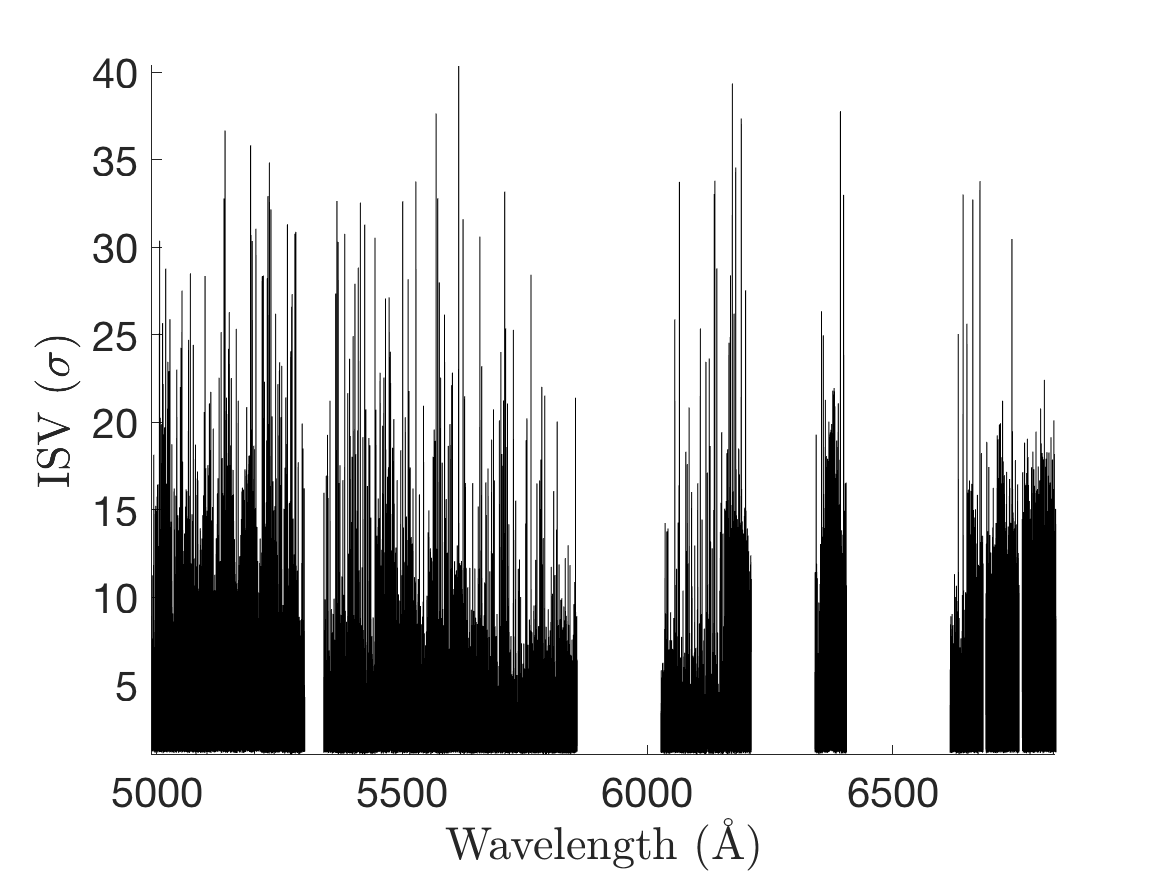
\includegraphics[width=0.69\textwidth]{GL667C_std_noise.png}}
    \subfloat[ISV of GL667C once the problematic observations were removed.]{\label{figGL667C_final}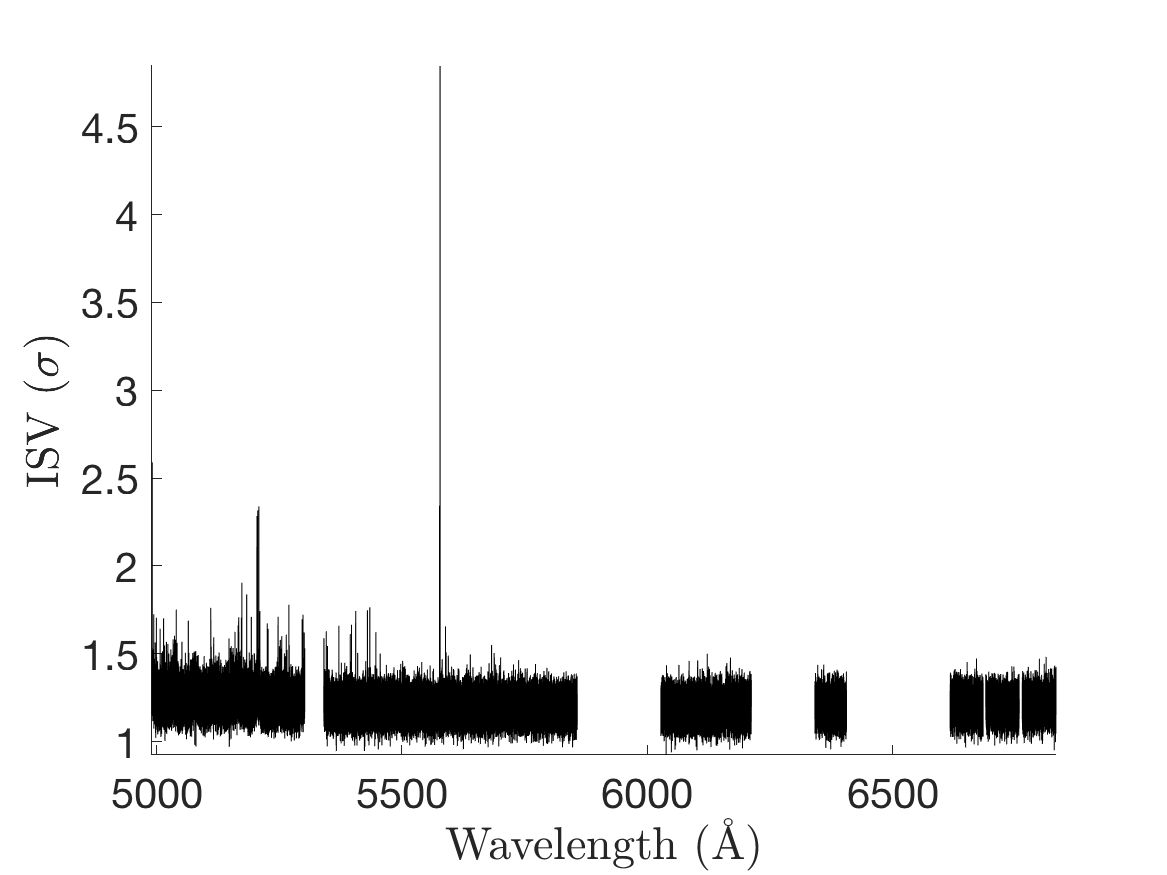
\includegraphics[width=0.69\textwidth]{GL667C_std.png}}
    \caption{}
    \label{figGL667C_ISV}
\end{figure}

Secondly the Doppler velocity needs to be no greater than $\pm$100 ms$^{-1}$ from the median. A Doppler velocity greater than 100 ms$^{-1}$ will either be incorrectly measured, or will be an observation of a nearby star that has been mistakenly observed. An example of this latter situation was GL667C. Comparing GL667C's ISV plot, Figure\,\ref{figGL667C_noise}, with a typical ISV plot such as  \ref{figLPV_TT}, the variance features of GL667C are not only much greater, but occur across almost all pixels. Investigation of the Doppler velocities (Figure\,\ref{figGL667C_RV}) shows 5 observations out of a total of 189, with substantially lower Doppler velocity ($\sim$4 kms$^{-1}$ lower). Looking at the spectra of these observations (Figure\,\ref{figGL667C_Int}), it was found that the 5 observations have fluxes up to 9 times greater than the rest. It is clear that these particular observations were not of GL667C. As GL667 is a triple-star system, these observations are most likely of GL667A or GL667B. Even though these 5 observations represent a small fraction of the total sample, their total fluxes are so much greater than the rest that this will produce statistically significant variation. Removing these observations produced an ISV much more inline with the rest of the sample (Figure\,\ref{figGL667C_final}).\\

\begin{figure}
	\hspace{-3cm}
	\captionsetup{width=.5\textwidth}
	\subfloat[Doppler Velocity of all observations of GL667C. The blue lines mark the $\pm$100 ms$^{-1}$ threshold from the median value.]{\label{figGL667C_RV}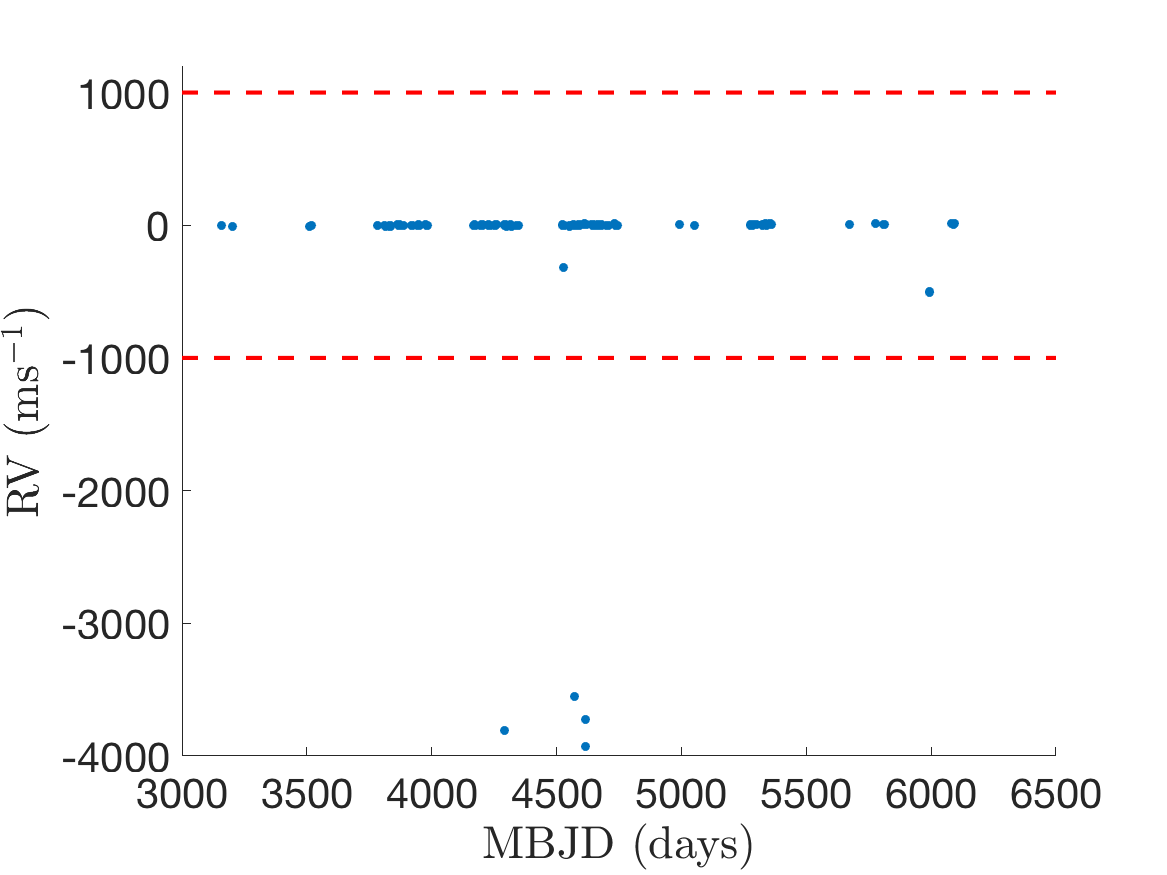
\includegraphics[width=0.69\textwidth]{GL667C_obs.png}}
    \subfloat[Intensity plot of the 40th order of GL667C for all 189 observations. Note the 5 observations with significantly greater fluxes than the rest.]{\label{figGL667C_Int}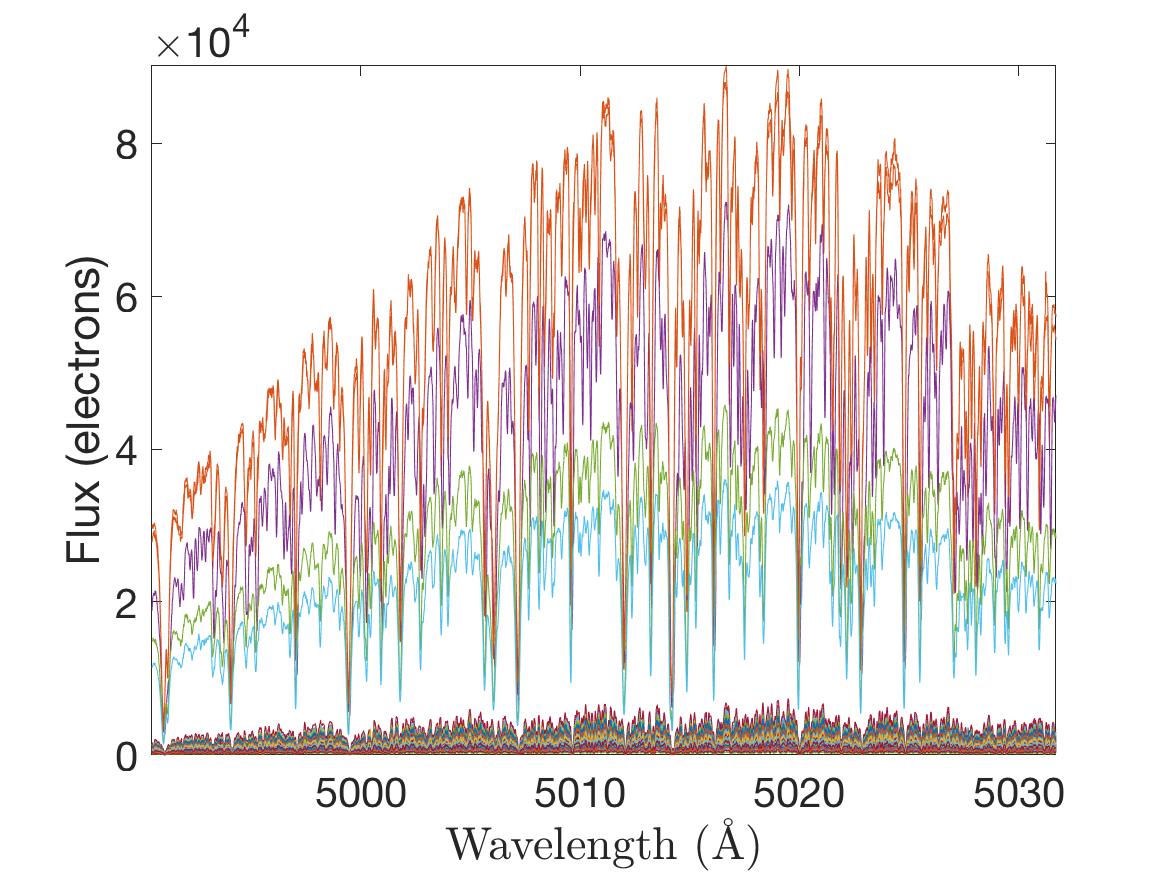
\includegraphics[width=0.69\textwidth]{GL667C_intensity.png}}
    \caption{}
    \label{figGL667C_Details}
\end{figure}

The only stars not to have this criterion applied were binaries, where the Doppler velocity will vary due to the orbital motion of the star. This can cause significant variation in Doppler velocity and so applying the 100 ms$^{-1}$ criterion would be problematic. As the number of binary stars in my sample was small, I visually inspected their Doppler velocities and removed any obvious outliers.\\

The procedure mean-weights the flux so that all observations have a mean flux of 1. For small changes in seeing, this is acceptable. Large changes in seeing, (or in the case of GL667C, a number of incorrect targets) will produce substantially higher or lower total flux. This will also cause non-stellar variations in the ISV that need to be removed. To check for this, I looked at the first `useful' HARPS order (40th). The mean flux across the order was taken for each observation, and the median of these was identified. All observations with a mean flux greater than 6-\,$\sigma$ from the median were removed.\\

The last criterion was specific to HARPS. In June of 2015, the fibres that connect the telescope to the spectrograph were upgraded \citep{2015LoCurto}. While this improved the quality of the spectra, the level of precision used in this method meant that data taken pre-fibre change could not be used with data taken post-change. As most of my data was taken before the change, all data taken after Julian date 2,457,165 were excluded.

\subsection{ISV features}
\label{secISVfeatures}
An ISV plot contains two main features - noise and variation features.\\

There is a level of variation across all pixels that ranges from 1.5\,-\,4\,$\sigma$. This comes from the signal-to-noise of the spectra and variable seeing and is essentially the `noise' of the ISV plot. The maximum level of this noise is dependent on the number of observations. Figure\,\ref{figNoise} compares GJ1256, which has 5 observations, with GL628, which has 164 observations. GJ1256 has a noise that goes up to 4\,$\sigma$, while GL628's noise only goes up to 1.5\,\,$\sigma$. While some of the difference can be explained by GL628 being brighter, and therefore having a greater signal-to-noise, the large number of observations in GL628 reduce the statistical significance of the observational noise, unlike GJ1256 which is dominated by this noise. Investigations of the number of observations and maximum noise level lead to the requirement of a minimum of 20 observations to ensure the noise does not go above 2\,$\sigma$.\\ 

\begin{figure}[!htb]
	\hspace{-3cm}
	\captionsetup{width=.8\textwidth}
	\subfloat[]{\label{figGL1256_noise}\includegraphics[width=0.69\textwidth]{GJ1256_std.png}}
    \subfloat[]{\label{figGL628_noise}\includegraphics[width=0.69\textwidth]{GL628_std.png}}
    \caption{ISV plots of GJ1256 (a) and GL628 (b). GJ1256 has a much higher level of `noise' than GL628 due to the low number of observations.}
    \label{figNoise}
\end{figure}

The variation of emission features in a star are seen in an ISV plot as pixels that have a variation greater than the surrounding noise levels. The greater the variation, the more that pixel has varied across the observations. For example, a pixel with an ISV of 3 means that there is a 3-$\sigma$ variation between all observations for that pixel. Statistically significant variations should indicate activity from an element that has a spectral line centred at that point but might not have been as easy to resolve as the traditional activity indicators.\\

Figures\,\ref{figLPV_TT_full} and \ref{figLPV_TT_zoom} highlight that a region of variance might appear to be a single pixel, but can actually comprise several pixels. When a emission feature varies, most of the spectral profile varies, not just the central wavelength. The ISV is showing how much each pixel is varying from observation to observation, and therefore a varying spectral line will cause variation across a range of pixels. A series of consecutive varying pixels is called a variance feature. Some variations above the noise are comprised of a single pixel. These were investigated and found to be variations from a single observation, indicating that this was most likely a cosmic ray that had not been properly filtered out when the spectra was processed. All variance features were expected to have a at least 3 pixels above the noise.\\

The profile of the variance features was found to be Gaussian, or in the case of multiple unresolved spectral features, a blend of Gaussians. Additionally the effect of cosmic rays and flares will cause significant variance features.

\subsection{Non-stellar spectral lines}
\label{secNonStellarLines}
HARPS spectra consists of 72 orders, however only some of them are useful for exoplanet Doppler velocity analysis. Section\,\ref{secSpectra} discusses in detail that M-dwarfs emit very little flux at blue wavelengths, and therefore a number of the blue HARPS orders contain very little useful information. Additionally, several orders are dominated by tellurics and molecular bandheads which will obscure any absorption lines used for Doppler velocity exoplanet detection (see Section\,\ref{SecRV}). As such, only 24 orders are `useful' for exoplanet detection - 40-56, 60-62, 65, and 69-71.\\

These remaining orders will still have some tellurics and sky emission lines that might vary at a sufficient level to appear on an ISV plot. It would be straight forward to identify the wavelengths at which these lines occur and ignore any variation at those points. However, due to their being at rest in the observers frame of reference, they will be shifted once the spectra is barycentrically corrected, meaning that each line will influence the variation of multiple pixels. These lines needed to be identified and their wavelengths examined to see their impact on the ISV.\\

Disentangling the terrestrial features from the stellar features in spectra can be difficult, especially in cool stars which have multiple features. For this reason a B-star spectra was used as it contains a relatively small number of absorption lines which, due to the high rotation rate of the star, are strongly rotationally broadened. Compared to the star, the rotation of the Earth is much smaller, leading to minimal rotational broadening in terrestrial features. This means the two sets of features, stellar and terrestrial, will be clearly different from each other, making it easier to identify the lines of interest.\\

I decided to use the ISV analysis on several B-stars to see if the tellurics cause variations on a scale above the noise. The reasoning for this was that a B-star has high signal-to-noise, much greater than the M-dwarfs observed by HARPS. The non-stellar lines present in both a B-star and M-star spectra will be more prominent in the B-star. Therefore if there is no significant ISV variation in a B-star spectra, then it will be even less significant for an M-dwarf and the ISV analysis will not have to account for their presence in the spectra.\\

There were several selection criteria for the B-stars. First, to compare like with like, they had to be observed by HARPS. This means the instrument and data reduction would be the same as for the M-dwarfs. This immediately limits the number of candidates as HARPS was designed to detect exoplanets. While it is possible for exoplanets to orbit B-stars, it is less likely. As such, the number of B-stars observed by HARPS will be limited.\\

Secondly the star needs to have a high rotational velocity. B-stars are known to be among the fastest rotators, however some will have a high orbital inclination with respect to the Earth, and the observations will be dominated by the poles, which rotate slower, producing prominent absorption lines that would normally by strongly broadened. For example, compare the spectra of HD148605 to HD149438.\\

\begin{figure}
	\hspace{-3cm}
	\captionsetup{width=.8\textwidth}
    \subfloat[HD148605]{\label{figHD148605_spectra}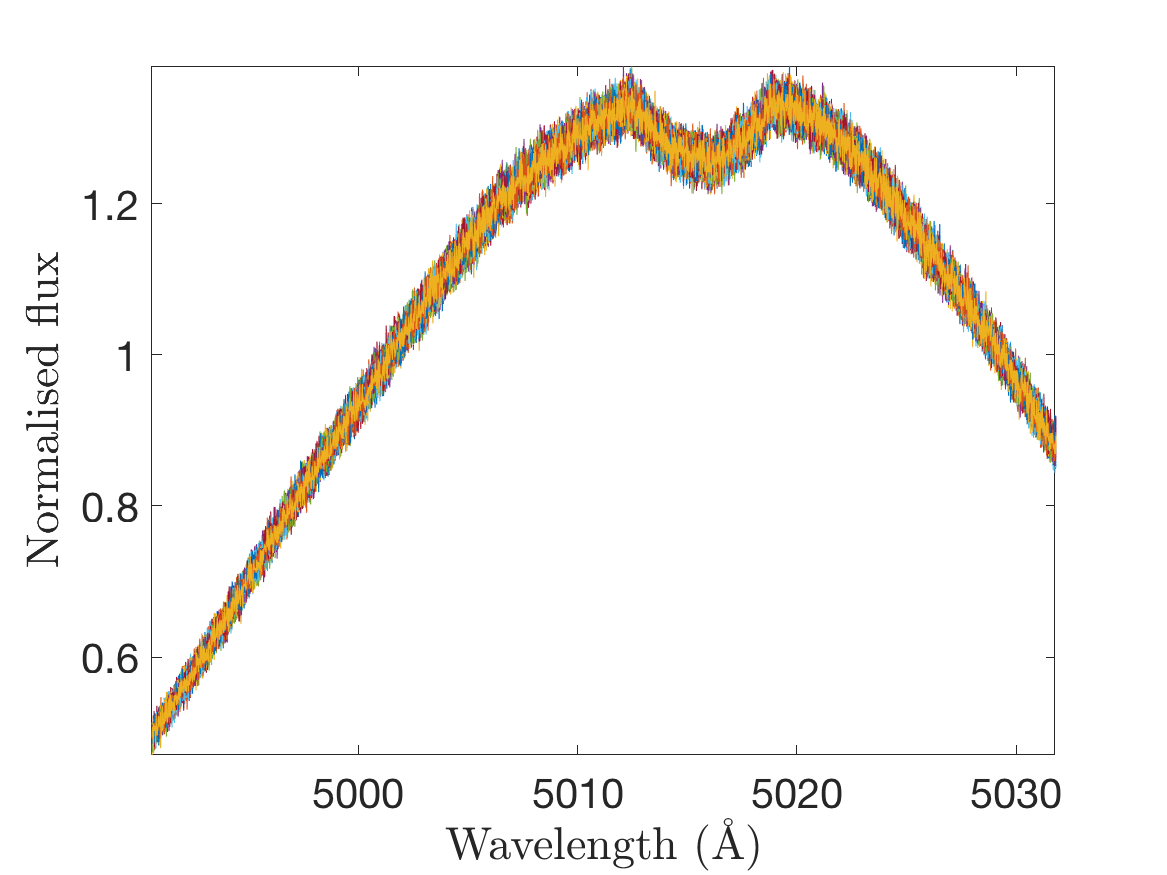
\includegraphics[width=0.69\textwidth]{HD148605_broad_lines.png}}
    \subfloat[HD149438]{\label{figHD149438_spectra}\includegraphics[width=0.69\textwidth]{HD149438_sharp_lines.png}}
    \caption{Spectra of HD148605 and HD149438. Note that HD148605 has broad absorption features, as is expected from a highly rotating star, while HD149438 has multiple features that are stronger and narrower than those seen in HD148605.}
    \label{figBstar_spectra}
\end{figure}

While HD148605 has broad absorption features expected of a highly rotating B-star, HD149438 has features more characteristic of a cooler star, stronger lines that are less broadened. While late B-stars will start to feature thinner and deeper spectral features than their earlier counterparts, HD149438 is classified as B0.2, making this explanation unlikely. Studies of HD149438 have measured its $vsini$ to be 7-9\,kms$^{-1}$, well below the expected levels of an early B-star. The ISV plot for HD149438 (Figure\,\ref{figHD149438_ISV}) shows significant variation coming from the unbroadened stellar features, making it difficult to see the effect (if any) of the tellurics present.\\

\begin{figure}
	\centering
	\captionsetup{width=.8\textwidth}
    \includegraphics[width=0.8\textwidth]{HD149438_comparison_b.png}
    \caption{ISV plot of HD149438.}
    \label{figHD149438_ISV}
\end{figure}

To properly align the spectra, both the Barycentric motion and the radial velocity of the star need to be corrected. For B-stars this is difficult as the main advantage of them for this work, broad stellar features, makes it difficult to measure accurate radial velocities. This is significant in multiple-star systems as the radial velocity of the star in will be much greater, meaning that it needs to be taken into account for the analysis to work. As such, I only selected single stars.\\

\begin{figure}
	\centering
	\captionsetup{width=.8\textwidth}
    \includegraphics[width=0.8\textwidth]{HD134481_comparison_b.png}
    \caption{ISV plot of HD134481 taken from 16 observations.}
    \label{figHD134481_noise}
\end{figure}

The last criterion was that the star needed to have sufficient observations to ensure a reasonable noise level (see Section\,\ref{secISVfeatures}). The argument stands if the noise level is reasonable, while too few observations will inflate the noise and will weaken the legitimacy of the argument. An example of this is HD134481 which had only 16 observations. The baseline noise in Figure\,\ref{figHD134481_noise} is $\sim$\,2, much greater than normal. Due to small number statistics, small variations in the flux from observation-to-observation for a particular pixel will have a significant ISV value due to the small number of data points. Any arguments as to the strength of telluric variations compared to the baseline noise would be invalid if the noise was inflated due to a low number of observations.\\

\begin{figure}
	\centering
	\captionsetup{width=.8\textwidth}
    \includegraphics[width=0.8\textwidth]{HD148605_comparison_b.png}
    \caption{ISV plot of HD148605. Note the lack of any significant variation above the baseline noise.}
    \label{figHD148605}
\end{figure}

An example of a star found to fit all these criteria is HD148605. As can be seen in Figure\,\ref{figHD148605}, there is no significant variation. This suggests that the effect of telluric lines are minimal to the point that they should not cause variations in the spectra of an M-dwarf to any level above the baseline noise.

\subsection{Cosmic ray removal}
\label{secCosmic}
As the ISV is analysing the change in flux from observation-to-observation, the effect of cosmic rays hitting the CCD will generate a strong emission feature in one observation that is expected to not be seen in subsequent observations. Despite its presence in only one observation, the intensity of this feature will produce a variation feature in an ISV plot of significant intensity. Obviously this is a false-positive that needs to be removed. While there are several methods for removing these rays from the spectra, I found that the method of determining the ISV also allows for the detection and removal of cosmic rays.\\

One of the final steps in producing the ISV was $I_{var}$ (Figure\,\ref{figLPV_thevar}), which is the residuals of each mean-normalised spectra and the mean of the mean-normalised spectra, divided by the uncertainties. This is essentially showing how, for a particular pixel, each observation varies from the mean of all the observations for that pixel.\\

I identified all pixels, across every observation, that had a $I_{var}$ value greater than 5 sigma. These points will include both cosmic rays and actual stellar variations. To distinguish between these two features I assumed that for each pixel a cosmic ray would present as a single high variation observation, with the previous and subsequent observations having a variation below 5 sigma, while a stellar variation would consist of multiple consecutive observations with a high variation. There is the chance that multiple cosmic rays could strike the same pixel on the CCD in consecutive observations, but that is statistically low, and any cosmic rays that are left in because of this assumption can be filtered out in later stages.\\

This left a list of pixels in specific observations that are expected to be cosmic rays and the spectra needed to be cleaned of them. I then replaced those pixel's values with the corresponding values from the mean of the mean-normalised spectra, $I_{mean}$. Being overly cautious, I also replaced the pixels either side of the cosmic ray affected pixel.\\

However this method produced issues with the ISV. As the ISV is determined from how the mean-normalised spectra changes over time, and that mean-normalised spectra is generated from all the spectra, altering the shape of the spectra also alters the mean-normalised spectra and therefore has a significant effect on the ISV. Comparing the black and blue lines in Figure\,\ref{figGL54.1_cosmic_comparison} highlights this. The blue line is the ISV for spectra with no cosmic cleaning, while the black is the ISV of spectra cleaned by the process discussed above. The cleaning routine has `flattened' out the ISV in the regions in between features, resulting in the removal of wings of most of the features.\\

\begin{figure}
	\centering
	\captionsetup{width=.8\textwidth}
    \includegraphics[width=0.8\textwidth]{Gl54_1_cosmic_comparison.png}
    \caption{ISV plot of GL54.1 comparing the results of cleaning the spectra of cosmic rays (black line), versus using uncleaned spectra (blue line).}
    \label{figGL54.1_cosmic_comparison}
\end{figure}

Looking at the spectra that generated these two ISV's shows that the cleaning process's criteria will remove those points that fit the criteria, while leaving all points just outside of the criteria unchanged. This causes these almost vertical slices in the spectra that are seen as similar vertical slices in the ISV. Reducing the threshold for identifying the cosmic rays would improve this, however it would also remove genuine stellar variations.\\

\begin{figure}
	\hspace{-2cm}
	\captionsetup{width=.8\textwidth}
    \subfloat[HD149438]{\label{figGL54.1_cosmic_clean}\includegraphics[width=0.69\textwidth]{Gl54_1_cosmic_clean.png}}
    \subfloat[HD148605]{\label{figGL54.1_cosmic_no_clean}\includegraphics[width=0.69\textwidth]{Gl54_1_cosmic_no_clean.png}}
    \caption{Spectra of GL54.1 used to produce the ISV plots shown in Figure\,\ref{figGL54.1_cosmic_comparison}. (a) The cosmic ray cleaned spectra; (b) The uncleaned spectra.}
    \label{figCosmic_spectra}
\end{figure}

It was decided that the best way of dealing with cosmic rays was to not deal with them at all, at least not at this stage. Any alteration of individual spectra would result in a disrupted ISV, and it was easier to filter out the cosmic ray affected pixels after the ISV had been generated. For example, there are two variance features in Figure\,\ref{figGL54.1_cosmic_ISV}, one at $\sim$5031.64\AA, and the other at $\sim$5031.89\AA. The left feature is made up of only 5 data points and covers a narrow wavelength range. The spectra of M-dwarfs are not expected to contain such a narrow spectral feature by itself. This is most likely a cosmic ray and further analysis will exclude features like this. While the feature on the right is covers a much greater wavelength range and is much more Gaussian in shape, there is some doubts at to its nature. Looking at the spectra (Figure\,\ref{figGL54.1_cosmic_spectra}) shows that the variance feature is comprised of only one observation. The activity I was looking for was expected to be seen in multiple observations. This feature may be a cosmic ray, a flare, or a short term stellar variation that was not sufficiently sampled. Regardless, these features are not useful for this work and needed to be excluded from further analysis.\\
 
\begin{figure}
	\hspace{-2cm}
	\captionsetup{width=.8\textwidth}
    \subfloat[HD149438]{\label{figGL54.1_cosmic_ISV}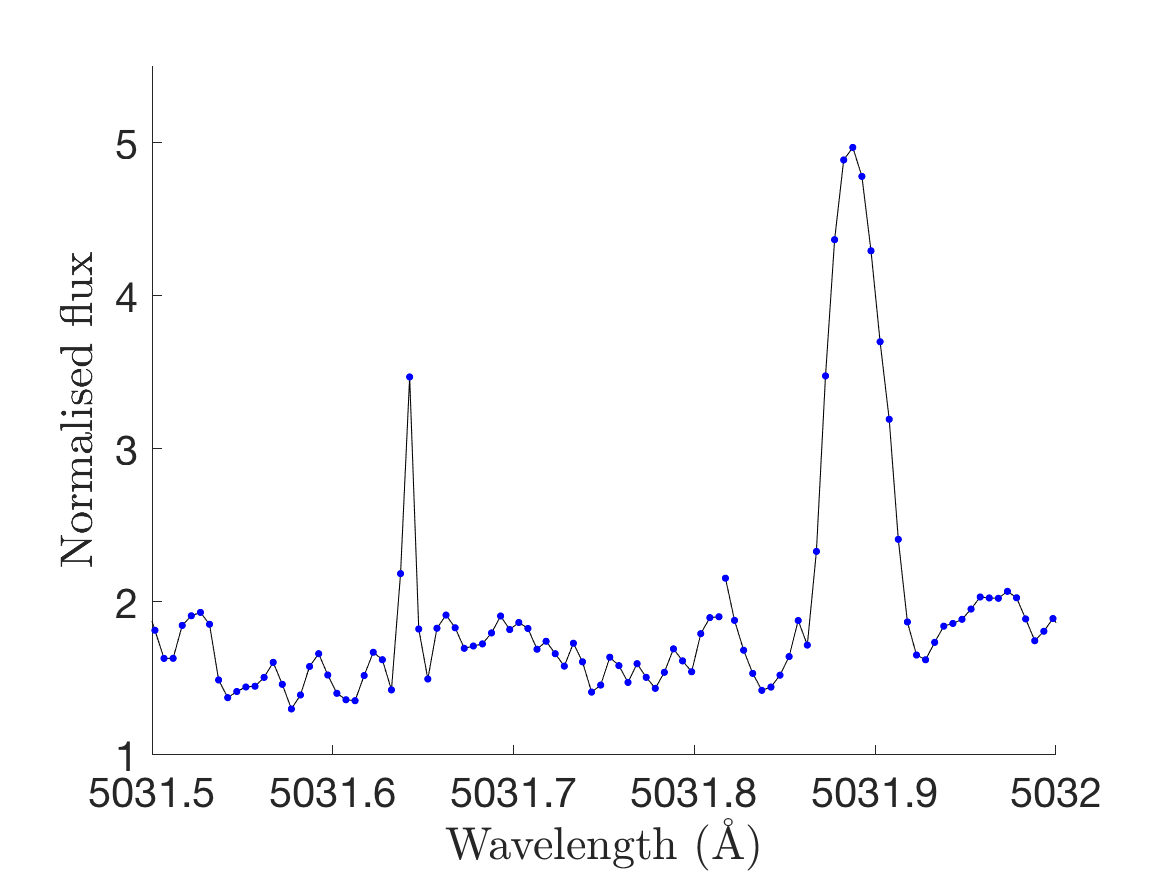
\includegraphics[width=0.69\textwidth]{Gl54_1_cosmic_ray_ISV.png}}
    \subfloat[HD148605]{\label{figGL54.1_cosmic_spectra}\includegraphics[width=0.69\textwidth]{Gl54_1_cosmic_ray_spectra.png}}
    \caption{Examples of probable cosmic rays that will be excluded from any analysis. (a) A region of the ISV plot of GL54.1 highlighting two expected cosmic rays; (b) The mean-normalised spectra at the same wavelength range. The break in the spectra at $\sim$5031.82\AA\:is the boundary between two HARPS orders.}
    \label{figCosmic_example}
\end{figure}

\section{Analysis of variance features}
Each variance feature should correspond to a varying spectral line. Identifying which elements correspond to each variance would give an indication about what activity the ISV is sensitive to, and tell us more about the variability in the star. To determine the statistically significant variance features, a baseline level needs to be determined. All features above that baseline can then be investigated. As mentioned in Section\,\ref{secISVfeatures}, the distribution of a variance feature is expected to be Gaussian or a blend of Gaussians. The central point of the Gaussian should correspond to the rest wavelength of the element causing the variation in the spectra.

\subsection{Determination of variation threshold}
Due to the variable level of noise, the deviation threshold cannot be set to one specific value as the `signal-to-noise' will vary depending on the number of observations. Looking at the ISV plots of the active M-dwarf subset stars, it was clear that the threshold should be a set amount above the noise of the ISV. Each order will have a varying average noise level, so any baseline value would have to determined across all the orders. Therefore I combined the variance across all orders and used the distribution of variance to determine the baseline noise.\\

\begin{figure}
    \hspace{-3cm}
    \captionsetup{width=.5\textwidth}
    \subfloat[A histogram of the variance across all wavelengths for GL551. The plot is zoomed in to highlight the range of ISV values around the noise. To determine the baseline noise level, the 95th percentile was determined (in red).]{\label{figGL551_hist}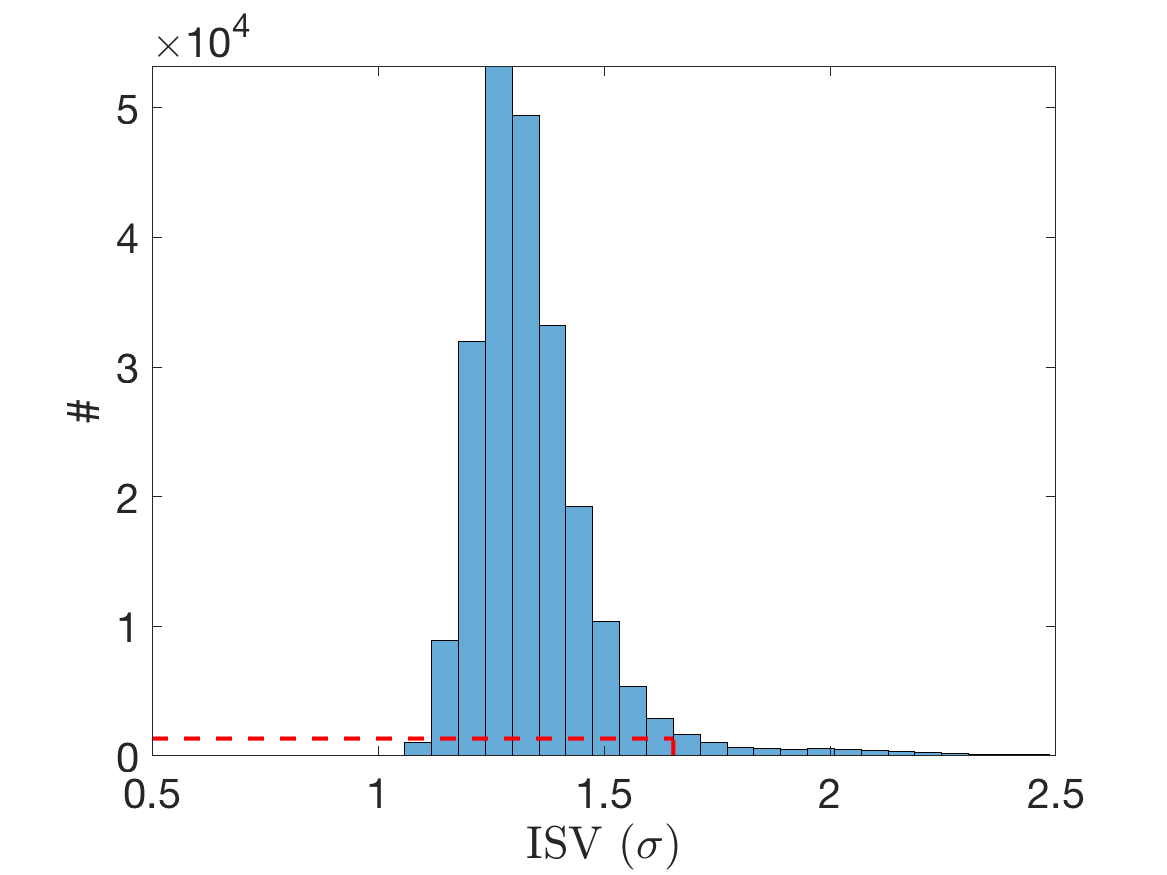
\includegraphics[width=0.69\textwidth]{GL551_Hist.png}}
    \subfloat[An ISV plot of GL551 with the baseline determined from the histogram in \ref{figGL551_hist} overplotted in red. The threshold is then 1\,$\sigma$ greater than this baseline (in blue).]{\label{figGL551_thresh}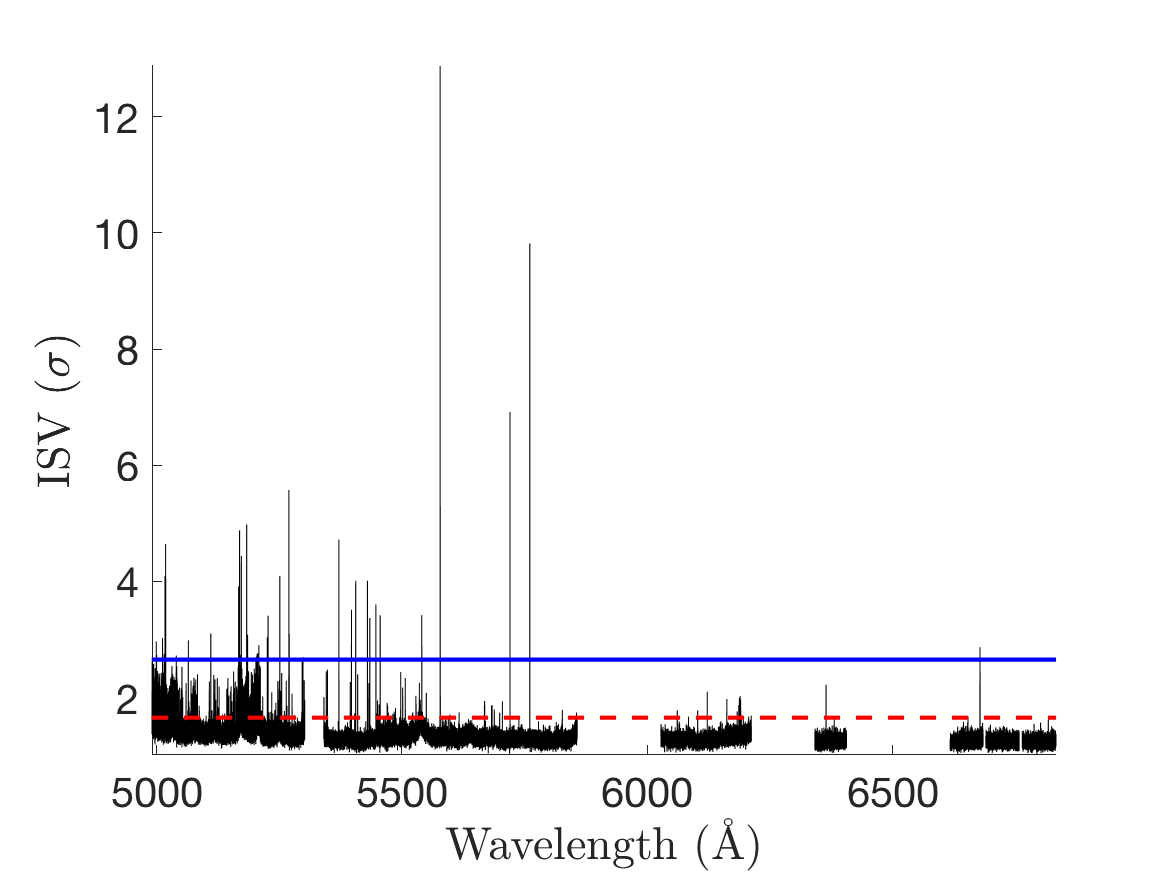
\includegraphics[width=0.69\textwidth]{GL551_TT.png}}
    \caption{}
    \label{figbaseline}
\end{figure}

Figure\,\ref{figGL551_hist} shows the distribution of variance for GL551 from 0.5-2.5. As the noise will be the bulk of the variance, it will make up the majority of the distribution and the baseline can be determined from this. The 95th percentile of the distribution was taken as the baseline noise level. From the distribution plot it can be seen that the baseline for GL551 was 1.65. This baseline is overplotted in red onto the ISV of GL551 in Figure\,\ref{figGL551_thresh} and it can be seen that this method does a sufficient job of determining an average noise baseline across all orders. To ensure that the threshold was clear of the noise, it was initially decided to only select variances greater than the baseline plus 1\,$\sigma$. This is the blue line in Figure\,\ref{figGL551_thresh}. All variances above this threshold would be considered significant enough to be actual stellar variation, and not noise. However this 1\,$\sigma$ above the noise threshold was found to select few spectra lines. Too high a threshold and only the strongest of elements, such as neutral iron and magnesium, will be detected, with several elements present in M-dwarf spectra below the threshold. Too low a threshold and the profile of the variance features will be dominated by the noise, distorting the expected Gaussian shape and making it more difficult to fit a Gaussian to. For example, compare the variance features of Figures\,\ref{figGL699_good} and \,\ref{figGL699_bad}. Figure\,\ref{figGL699_good} has a variance feature produced by neutral iron, which is a strong emitter, and produces a high signal-to-noise variance feature. The shape of the feature is dominated by the signal and therefore is a lot closer to a Gaussian distribution than Figure\,\ref{figGL699_bad}. This variance feature is much more distorted from the expected Gaussian shape due to the noise. This feature is produced by neutral titanium which will not emit as strongly as iron. I investigated where is the best medium between selection of elements and confidence in the signal, and a threshold of 0.5\,$\sigma$ above the noise was found to include most of the elements expected in M-dwarf spectra, while staying sufficiently above the noise.\\

\begin{figure}
	\hspace{-2cm}
	\captionsetup{width=.8\textwidth}
    \subfloat[]{\label{figGL699_good}\includegraphics[width=0.69\textwidth]{GL699_good_clump.png}}
    \subfloat[]{\label{figGL699_bad}\includegraphics[width=0.69\textwidth]{GL699_bad_clump.png}}
    \caption{ISV variance features of GL699. (a) An example of a strongly emitting element prodcuing a high signal-to-noise variance feature. (b) This variance feature is much more distorted from the expected Gaussian shape due to the noise.}
\end{figure}

\subsection{Selection of variance features}
\label{secVarFeature}
Applying this threshold identified the points of the variance features of significance. Gaussians were to be fitted to the points of each feature, however due to the varying signal-to-noise discussed above, the shape of a variance feature will not be perfectly Gaussian. To fit only to the points above the threshold would generate a poor fit. Instead, I extended the selection of data points down to the last data point that is just above the baseline noise, so long as the ISV does not increase in magnitude before passing this threshold. For example the blue crosses in Figure\,\ref{figLHS1723_clump} are extended to near the blue dashed horizontal line that represents the top of the baseline noise. However the ISV increases from the next points out. As I needed to fit only one feature, and the gradient of the feature was reversing, this could possibly include points from another feature which would lead to a poor fit.\\

\begin{figure}
	\centering
	\captionsetup{width=.8\textwidth}
    \includegraphics[width=0.8\textwidth]{LHS1723_clump_selection.png}
    \caption{one of the variance features found in LHS1723. The red crosses are the points above the threshold (red dashed line) that determined this feature to be of significance. The blue crosses are the points between the threshold and the top of baseline noise (blue dashed line).}
    \label{figLHS1723_clump}
\end{figure}

Not all the variance features will be due to activity. As mentioned in Section\,\ref{secCosmic}, the ISV will include variation from cosmic rays and flares. Additionally not all of the variations will be due to spectral variability. Because of this, I used three criteria to identify the `real' variance features. The first criterion was that the wavelength range that the variance feature spans must be greater than the minimum wavelength range that HARPS is capable of resolving (0.06\AA). Any feature smaller than this would be an artifact of the data reduction and not actual stellar variability. The second criterion was a check for cosmic rays. A cosmic ray would create a strong emission feature that could generate a significant ISV variance feature. As they are a result of a highly accelerated particle hitting the CCD, there will often only be one CCD pixel influenced. This means that the cosmic ray should span a very small wavelength range and will be removed by the first criterion. However, in the case that it hits multiple CCD pixels and spans a larger wavelength range, it can be identified due to it affecting only one observation. I looked at the $I_{var}$ for wavelength range the variance feature spans and checked how many observations were more than 2\,$\sigma$ from the median. A real stellar variation will have multiple observations above 2\,$\sigma$, that will combined to produce a variance feature above the threshold. A cosmic ray will most likely only have one, very strong, variation, and will be excluded. Lastly the third criterion was that there had to be at least one element, known to be present in M-dwarfs, that would produce a spectral line within the wavelength range of the variance feature. For this I used a line list compiled and used by the GALAH survey\,\citep{2015DeSilva}, which can be seen in Table\,\ref{tabLineList}. \\

\subsection{Elemental identification of variance}
The majority of variance features come from a single element and will be roughly Gaussian in shape. However, multiple unresolved spectral lines will form a blended feature in the spectra, therefore it is reasonable to expect that they will form a blended variance feature as well. Inspection of the variance features agrees with both of these assumptions. Therefore, to identify the elements producing the variability seen in an ISV plot, a combination of Gaussians needed to be fitted to each variance feature and the central wavelength of the Gaussian should correspond with the central wavelength of the spectral line that it corresponds to.\\

The number of Gaussians required to fit to the variance feature was determined by finding the number of `peaks' in the data that are separated by at least two data points. A non-linear least-squares fitting routine was used to fit the sum of the Gaussian to the data. Initial and boundary conditions were based off the `peak' properties and the properties of the variance feature as a whole.\\

\begin{figure}
    \centering
    \captionsetup{width=.8\textwidth}
    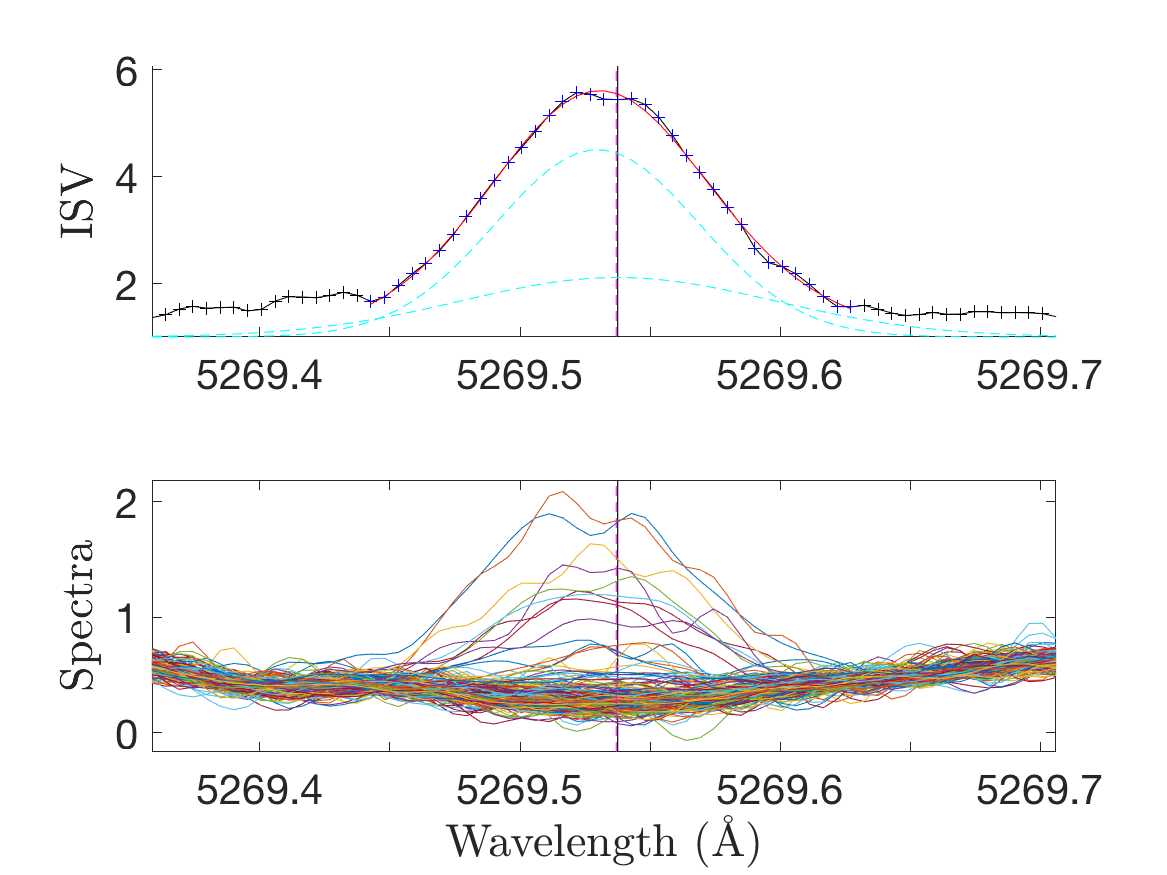
\includegraphics[width=0.8\textwidth]{GL551_Gaussian_fit_good.png}
    \caption{An ISV plot of a variance feature present in the spectra of GL551, with the mean-normalised spectra producing the ISV below. The cyan dashed lines are the Gaussians that combine into the red line which is the best fit to the feature. The magenta vertical dashed line represents the position of the nearest line from the GALAH line list, and the black vertical line is the central wavelength of the Gaussian.}
    \label{figGaussian_fitting_good}
\end{figure}

A non-linear least-squares fitting routine was used to fit a Gaussian to each feature and the central point of this Gaussian was considered the central wavelength of the feature. For example, Figure\,\ref{figGaussian_fitting_good} shows a variance feature, with a fitted Gaussian in cyan. From the GALAH line list, a neutral iron spectral line is present at 5269.537\,\AA and the Gaussian central wavelength is at 5269.538\,\AA. In the case of a variance feature with a more distorted distribution, either the noise is dominating the signal, or there are multiple components of this feature, where some, but not all, will be due to a spectral line. For example, Figure\,\ref{figGaussian_fitting_bad} where the distribution is very noisy and multiple Gaussians have been fitted. The fit is poor, however one of the Gaussians produced lies very close to the known spectral line (within 0.03\,\AA). Due to the high precision of the line list and the influence of the noise on the distribution of the variance feature, if the spectral line fell within the HWHM of the Gaussian, I considered that to be a confirmation.\\

\begin{figure}
    \centering
    \captionsetup{width=.8\textwidth}
    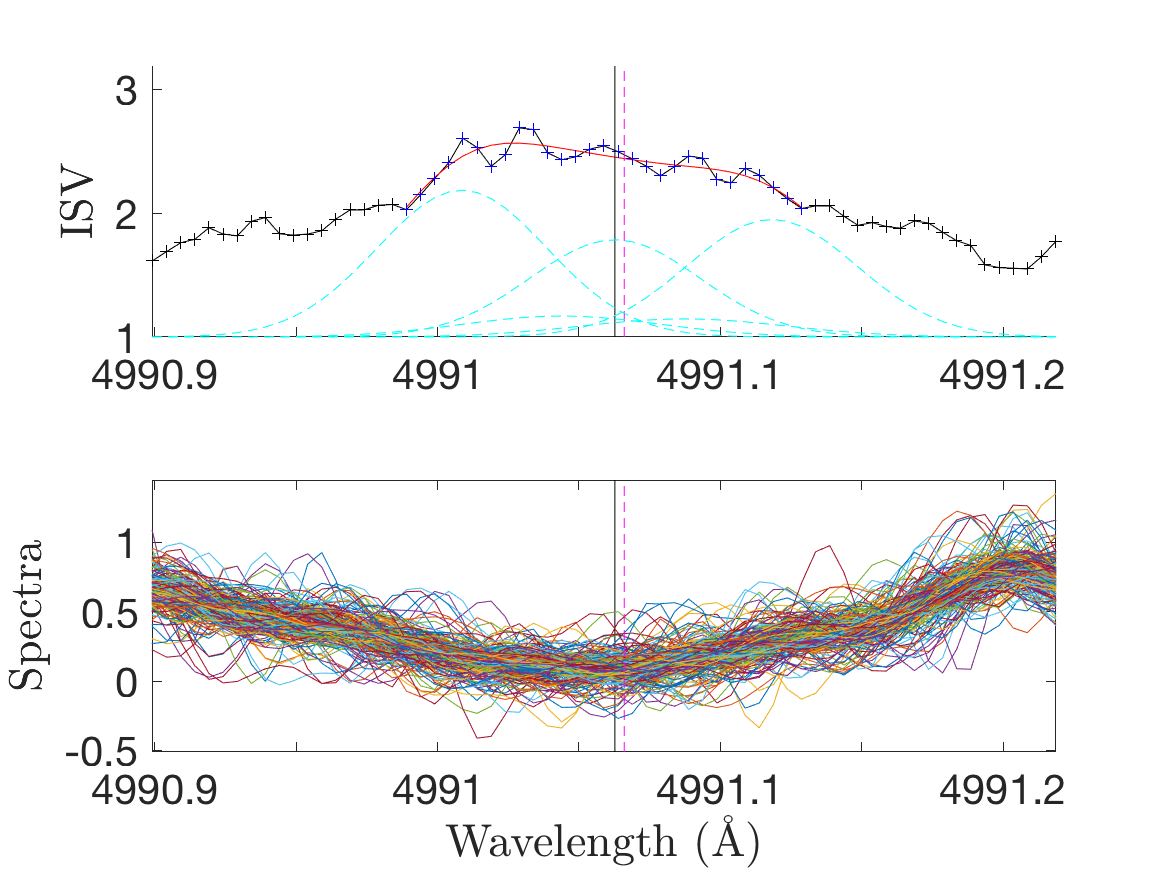
\includegraphics[width=0.8\textwidth]{GL551_Gaussian_fit_bad.png}
    \caption{An ISV plot of a variance feature comprised of several Gaussians.}
    \label{figGaussian_fitting_bad}
\end{figure}

\subsection{Selection of active stars}
All the HARPS M-dwarfs (Table\,\ref{tabHARPS}) were analysed using the criteria discussed in Section\,\ref{secVarFeature}. About half the sample of stars contained no variance features that passed the criteria, suggesting that they are not very active. I selected a subsample of the stars that contained multiple variance features (more than 3). I observed that the stars that contained three or less variance features had features barely above the threshold and fitted poorly. The sample of stars of stars with many variance features was sufficiently large to justify the exclusion of these poor quality stars. The active M-dwarf subsample is presented in Table\,\ref{tabMsample}.\\ 

\begin{sidewaystable}
    \begin{tabular}{|r|c|c|c|c|c|c|c|c|c|}
    \hline
    Designation & Sp. Type & Ra & Dec & Parallax & Observations & MBJD start & MBJD finish & Nights & Range\\
     & & hrs & \degree & mas & (\#) & (days) & (days) & (days) & (years) \\
     \hline
GJ2066 & M2 &08 16 07.9814381592 & 01 18 09.267240612 & 111.8419 & 83 & 2987.79 & 7115.54 & 80 & 11.3\\    
GL105B & M3.5 &02 36 15.2666844128 & 06 52 17.924295081 & 138.4637 & 22 & 2986.61 & 5414.94 & 22 & 6.6\\   
GL191 & M1 &05 11 40.5893175460 & -45 01 06.353955874 & 254.2263 & 96 & 2985.74 & 6667.8 & 48 & 10.1\\     
GL213 & M4 &05 42 09.2672965388 & 12 29 21.611736198 & 172.7068 & 46 & 2986.74 & 7116.48 & 46 & 11.3\\     
GL273 & M3.5 &07 27 24.49975 & 05 13 32.8332 & 262.98 & 225 & 2986.77 & 7144.47 & 198 & 11.4\\             
GL299 & M4.5 &08 11 57.5595749358 & 08 46 22.983154927 & 145.4757 & 22 & 2986.79 & 6321.7 & 22 & 9.1\\     
GL300 & M3.5 &08 12 40.8887006440 & -21 33 06.982376130 & 123.2204 & 39 & 2986.8 & 5309.48 & 37 & 6.4\\    
GL357 & M2.5 &09 36 01.6372518187 & -21 39 38.878281901 & 105.883 & 49 & 3815.72 & 6336.79 & 49 & 6.9\\    
GL358 & M3 &09 39 46.3688775322 & -41 04 03.201224127 & 104.1538 & 34 & 3669.84 & 6325.84 & 34 & 7.3\\     
GL388 & M5 &10 19 36.2808024653 & 19 52 12.014037746 & 201.3683 & 46 & 2986.86 & 6659.85 & 39 & 10.1\\     
GL447 & M4 &11 47 44.3968668170 & 00 48 16.404931305 & 296.3073 & 131 & 3578.46 & 7138.65 & 126 & 9.7\\    
GL54.1 & M4 &01 12 30.6367741360 & -16 59 56.361313690 & 269.3628 & 89 & 2986.6 & 7003.58 & 87 & 11\\      
GL551 & M5.5 &14 29 42.9451234609 & -62 40 46.170818907 & 768.5004 & 257 & 3152.6 & 6667.83 & 89 & 9.6\\   
GL581 & M3 &15 19 26.8271336166 & -07 43 20.190958776 & 158.7492 & 243 & 3152.71 & 6061.68 & 236 & 8\\     
GL628 & M3 &16 30 18.0582010683 & -12 39 45.323235188 & 232.2095 & 164 & 3158.67 & 7145.83 & 158 & 10.9\\  
GL674 & M3 &17 28 39.9455601300 & -46 53 42.693246243 & 219.8012 & 178 & 3158.75 & 7140.9 & 172 & 10.9\\   
GL678.1A & M1 &17 30 22.7281969656 & 05 32 54.663804222 & 98.8491 & 123 & 3159.73 & 7142.83 & 120 & 10.9\\ 
GL693 & M3.5 &17 46 34.2335493264 & -57 19 08.560062398 & 169.8613 & 128 & 3201.65 & 7145.85 & 124 & 10.8\\
GL699 & M4 &17 57 48.4997994034 & 04 41 36.111354228 & 547.4506 & 232 & 4194.89 & 6428.92 & 114 & 6.1\\    
GL754 & M4.5 &19 20 47.9834943463 & -45 33 29.629210788 & 169.0921 & 122 & 3154.83 & 6871.69 & 116 & 10.2\\
LHS1723 & M4 &05 01 57.4261049715 & -06 56 46.371875101 & 186.0231 & 124 & 2986.72 & 7103.52 & 117 & 11.3\\
\hline
    \end{tabular}
    \caption{HARPS M-dwarfs found to have significant variations in their ISV plots. MBJD is the Julian date minus 2,450,000 days. Nights is the total number of nights each star was observed, and Range is the time span in years for all observations.}
    \label{tabMsample}
\end{sidewaystable}https://www.overleaf.com/project/5ce3bf5fb0676376af3ce3a2
\section{Results}
\begin{figure}
    \hspace{-2cm}
    \captionsetup{width=.8\textwidth}
    \includegraphics[width=0.59\textwidth]{ISV_results_histogram_1.png}
    \includegraphics[width=0.59\textwidth]{ISV_results_histogram_2.png}\\
    \includegraphics[width=0.59\textwidth]{ISV_results_histogram_3.png}
    \includegraphics[width=0.59\textwidth]{ISV_results_histogram_4.png}
    \caption{Histograms of each spectral line in the GALAH line list and the percentage of the active star sample that have those lines varying according to ISV analysis. The plot underneath shows the wavelengths of the GALAH line list (red) and the HARPS wavelengths (blue).}
    \label{figISV_wavelength}
\end{figure}
The elements found to correlate with a variance feature are collated in Table\,\ref{tabElementFull}. A summary of the results (Table\,\ref{tabElementFrequency}) shows that the majority of varying elements are neutral metals such as iron, titanium, calcium and chromium. The only ionised element found to be varying is iron. From Figure\,\ref{figISV_wavelength} it can be seen that the most common wavelength regions to see activity are at the bluer end of the spectrum, while the red end sees little activity. This is not surprising as there will be more flux at the blue wavelengths, meaning that the activity is more prominent, but also due to the lack of wavelength coverage due to entire orders being dominated by telluric lines. As discussed in Section\,\ref{secNonStellarLines}, the tellurics will not produce variation of a scale noticeable by the ISV, however they are problematic for Doppler velocity measurements and regions dominated by these lines are avoided. As such, I have not investigated the activity in these regions as they are of no use for improving the precision of Doppler velocity measurements.

\begin{table}[]
    \centering
    \begin{tabular}{|c|c|c|}
    \hline
    Element & Frequency & Percentage \\
    \hline
    Fe 1 & 31 & 39.74 \\
    Ti 1 & 17 & 21.79 \\
    Ca 1 & 13 & 16.67 \\
    Cr 1 &  7 &  8.97 \\
    Fe 2 &  4 &  5.13 \\
    Na 1 &  3 &  3.85 \\
    Mg 1 &  2 &  2.56 \\
    Ni 1 &  1 &  1.28 \\
    \hline
    \end{tabular}
    \caption{The number of wavelengths a particular varying element is found to be  within the subsample of active HARPS M-dwarfs.}
    \label{tabElementFrequency}
\end{table}

